\PassOptionsToPackage{table}{xcolor}

\documentclass[aspectratio=169]{beamer}

\usetheme{auriga}
\usecolortheme{auriga}
\setbeamersize{text margin left=2em,text margin right=2em}

\usepackage{fontspec}
\usepackage{xcolor}
\usepackage{enumitem}
\usepackage{makecell}
\usepackage{tabularx}
\usepackage[outputdir=build, newfloat]{minted}
\usepackage{unicode-math}
\usepackage{animate}
\usepackage{amsmath}
\usepackage{ulem}
\usepackage[russian]{babel}
\usepackage{xpatch,letltxmacro}

\LetLtxMacro{\cminted}{\minted}
\let\endcminted\endminted
\xpretocmd{\cminted}{\RecustomVerbatimEnvironment{Verbatim}{BVerbatim}{}}{}{}

\setminted{
  fontsize=\scriptsize,
  baselinestretch=1.5
}

% for vertical centering text in X column
\renewcommand\tabularxcolumn[1]{m{#1}}
\newcolumntype{C}{>{\centering\arraybackslash}X}

\setmainfont{PT Astra Serif}

\makeatletter
\AddEnumerateCounter{\asbuk}{\russian@alph}{щ}
\makeatother

\title{
  \huge{
    Индексы в PostgreSQL
  }
}
\author{Швалов Даниил К33211}
\institute{Университет ИТМО}
\date{2023}

\begin{document}

% change itemize default label
\def\labelitemi{---}

\frame{\titlepage}

\begin{frame}
  \begin{center}
    {\huge \textbf{Представим...}}
  \end{center}
\end{frame}

\begin{frame}
  \frametitle{Что такое индексы}

  \begin{columns}[onlytextwidth,c]
    \column{0.6\textwidth}

    \textbf{Индекс} --- это некоторая структура данных, которая повышает
    скорость операций поиска данных в таблице БД. Благодаря индексам можно
    находить нужную информацию быстрее, чем полным перебором.

    \vspace*{1em}

    Одним из примеров индексов в бытовой жизни является алфавитный указатель. Он
    представляет из себя список ключевых слов или фраз, используемых всюду в
    документе, который может помочь читателю быстро находить информацию.

    \column{0.4\textwidth}

    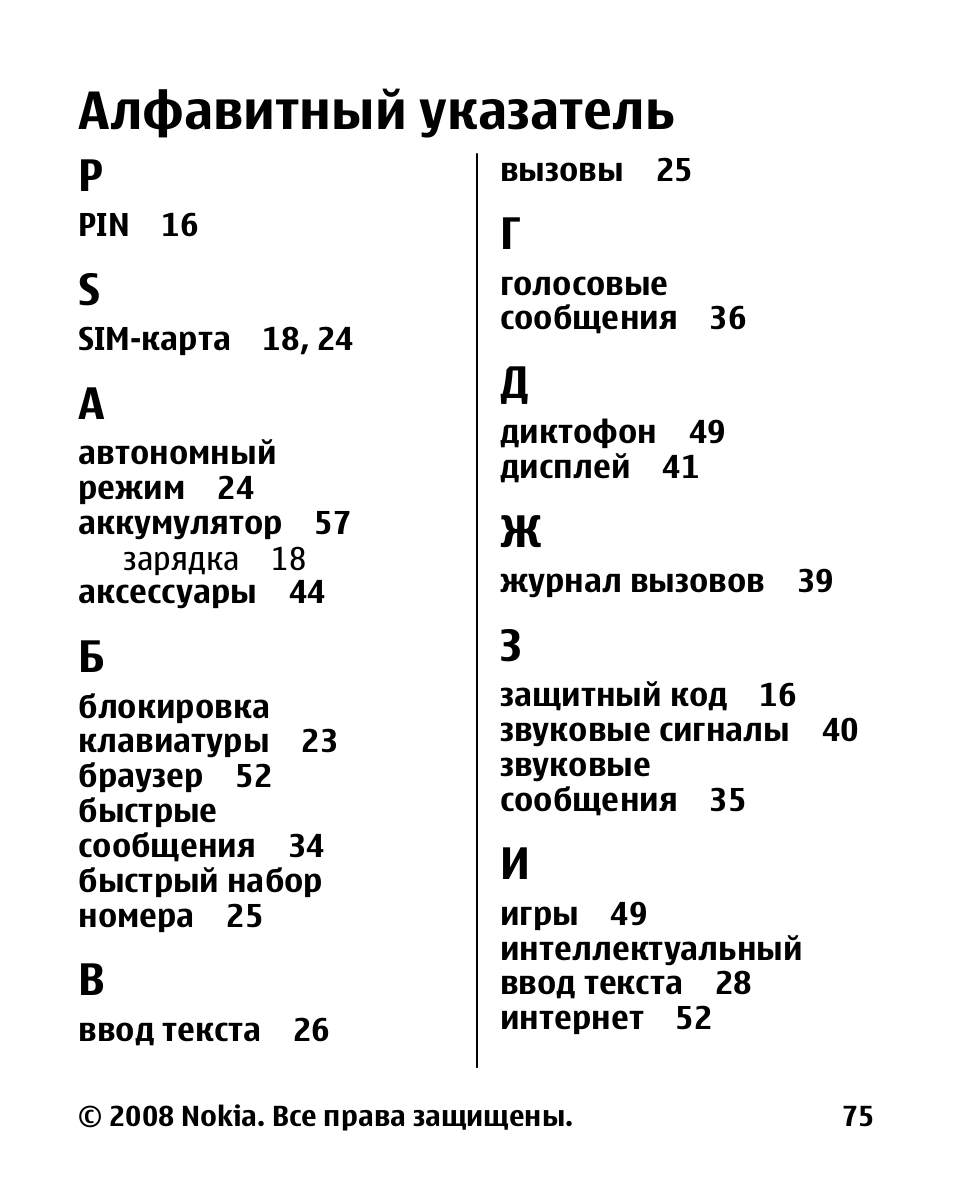
\includegraphics[width=\textwidth]{images/alphabetical-index.png}
  \end{columns}
\end{frame}

\begin{frame}
  \begin{center}
    {\huge \textbf{Как устроены индексы в \\ PostgreSQL}}
  \end{center}
\end{frame}

\begin{frame}
  \frametitle{Как хранятся строки таблиц}

  Каждая страница содержит заголовок (PageHeaderData), идентификаторы элементов
  (ItemId), элементы (Item) и особый раздел (Special).

  \vspace*{1em}

  Внутри каждого элемента лежит указатель на данный элемент, который состоит из
  номера страницы и индекса идентификатора элемента. Этот указатель обозначается
  как TID (Tuple ID).

  \vspace*{1em}

  \begin{center}
    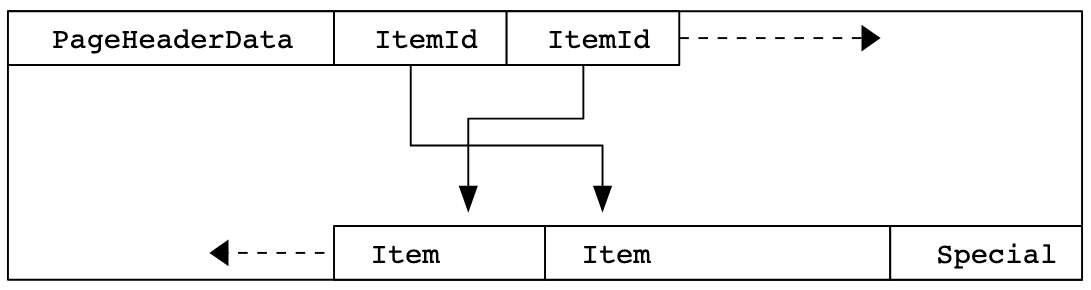
\includegraphics[width=\textwidth]{images/page.png}
  \end{center}
\end{frame}

\begin{frame}
  \vspace*{1em}
  \begin{center}
    {\LARGE \textbf{Основной принцип работы индексов}}

    \vspace*{1em}

    Индекс = соответствие некоторого ключа и TID

  \end{center}
\end{frame}

\begin{frame}[fragile]
  \frametitle{Что такое EXPLAIN}

  Синтаксис:
  \begin{minted}{sql}
EXPLAIN [ ANALYZE ] <OPERATOR>
  \end{minted}

  Пример использования:
  \begin{minted}{sql}
EXPLAIN 
SELECT * 
FROM some_table
WHERE b = 'q';
  \end{minted}

  Результат выполнения:
  \begin{minted}{text}
                               QUERY PLAN
----------------------------------------------------------------
 Seq Scan on some_table  (cost=0.00..1693.00 rows=1103 width=7)
   Filter: (b = 'q'::text)
(2 rows)
  \end{minted}
\end{frame}

\begin{frame}
  \frametitle{Виды сканирования}

  В PostgreSQL существуют следующие виды сканирования:
  \begin{itemize}
    \item последовательное сканирование или Seq Scan;
    \item индексное сканирование или Index Scan;
    \item сканирование по битовой карте или Bitmap Index Scan;
    \item исключительно индексное сканирование или Index Only Scan;
    \item сканирование по TID или TID Scan.
  \end{itemize}
\end{frame}

\begin{frame}[fragile]
  \frametitle{Пример индексного сканирования}

  Пример запроса:
  \begin{minted}{sql}
EXPLAIN SELECT * FROM some_table WHERE a = 123;
  \end{minted}

  \vspace*{1em}

  Результат выполнения:
  \begin{minted}{text}
                                    QUERY PLAN
-----------------------------------------------------------------------------------
 Index Scan using some_table_a_idx on some_table  (cost=0.29..8.31 rows=1 width=7)
   Index Cond: (a = 123)
(2 rows)
  \end{minted}
\end{frame}

\begin{frame}[fragile]
  \frametitle{Пример сканирования по битовой карте}

  Пример запроса:
  \begin{minted}{sql}
EXPLAIN SELECT * FROM some_table WHERE a < 1000;
  \end{minted}

  \vspace*{1em}

  Результат выполнения:
  \begin{minted}{text}
                                    QUERY PLAN
-----------------------------------------------------------------------------------
 Bitmap Heap Scan on some_table  (cost=20.07..475.62 rows=1004 width=7)
   Recheck Cond: (a < 1000)
   ->  Bitmap Index Scan on some_table_a_idx  (cost=0.00..19.82 rows=1004 width=0)
         Index Cond: (a < 1000)
(4 rows)
  \end{minted}
\end{frame}

\begin{frame}[fragile]
  \frametitle{Пример исключительно индексного сканирования}

  Пример запроса:
  \begin{minted}{sql}
EXPLAIN SELECT a FROM some_table WHERE a < 100;
  \end{minted}

  \vspace*{1em}

  Результат выполнения:
  \begin{minted}{text}
                                        QUERY PLAN
------------------------------------------------------------------------------------------
 Index Only Scan using some_table_a_idx on some_table  (cost=0.29..6.04 rows=100 width=4)
   Index Cond: (a < 100)
(2 rows)
  \end{minted}
\end{frame}

\begin{frame}[fragile]
  \frametitle{Пример сканирования по TID}

  Пример запроса:
  \begin{minted}{sql}
EXPLAIN SELECT * FROM some_table WHERE ctid = '(179,133)';
  \end{minted}

  \vspace*{1em}

  Результат выполнения:
  \begin{minted}{text}
                        QUERY PLAN
----------------------------------------------------------
 Tid Scan on some_table  (cost=0.00..4.01 rows=1 width=7)
   TID Cond: (ctid = '(179,133)'::tid)
(2 rows)
  \end{minted}
\end{frame}

\begin{frame}
  \vspace*{1em}
  \begin{center}
    {\huge \textbf{Создание индексов в PostgreSQL}}
  \end{center}
\end{frame}

\begin{frame}[fragile]
  \frametitle{Синтаксис создания индексов}

  Пример создания простого индекса:
  \begin{minted}{sql}
CREATE INDEX index_name ON table_name (column_name);
  \end{minted}

  \vspace*{1em}

  Пример создания индекса по нескольким столбцам:
  \begin{minted}{sql}
CREATE INDEX index_name ON table_name (col1, col2);
  \end{minted}

  \vspace*{1em}

  Пример создания уникального индекса:
  \begin{minted}{sql}
CREATE UNIQUE INDEX index_name ON table_name (column_name);
  \end{minted}
\end{frame}

\begin{frame}[fragile]
  \frametitle{Синтаксис создания индексов}

  Пример создания частичного индекса:
  \begin{minted}{sql}
CREATE INDEX index_name ON table_name (column_name)
WHERE column_name < some_value;
  \end{minted}

  \vspace*{1em}

  Пример создания индекса по выражению:
  \begin{minted}{sql}
CREATE INDEX index_name ON table_name (lower(column_name));
  \end{minted}

  \vspace*{1em}

  Пример параллельного построения индекса:
  \begin{minted}{sql}
CREATE INDEX CONCURRENTLY index_name ON table_name (column_name);
  \end{minted}
\end{frame}

\begin{frame}
  \vspace*{1em}
  \begin{center}
    {\huge \textbf{Типы индексов в PostgreSQL}}
  \end{center}
\end{frame}

\begin{frame}
  \vspace*{1em}
  \begin{center}
    {\huge \textbf{B-Tree индекс}}
  \end{center}
\end{frame}

\begin{frame}
  \frametitle{B-Tree индекс: поиск по равенству}

  \centering
  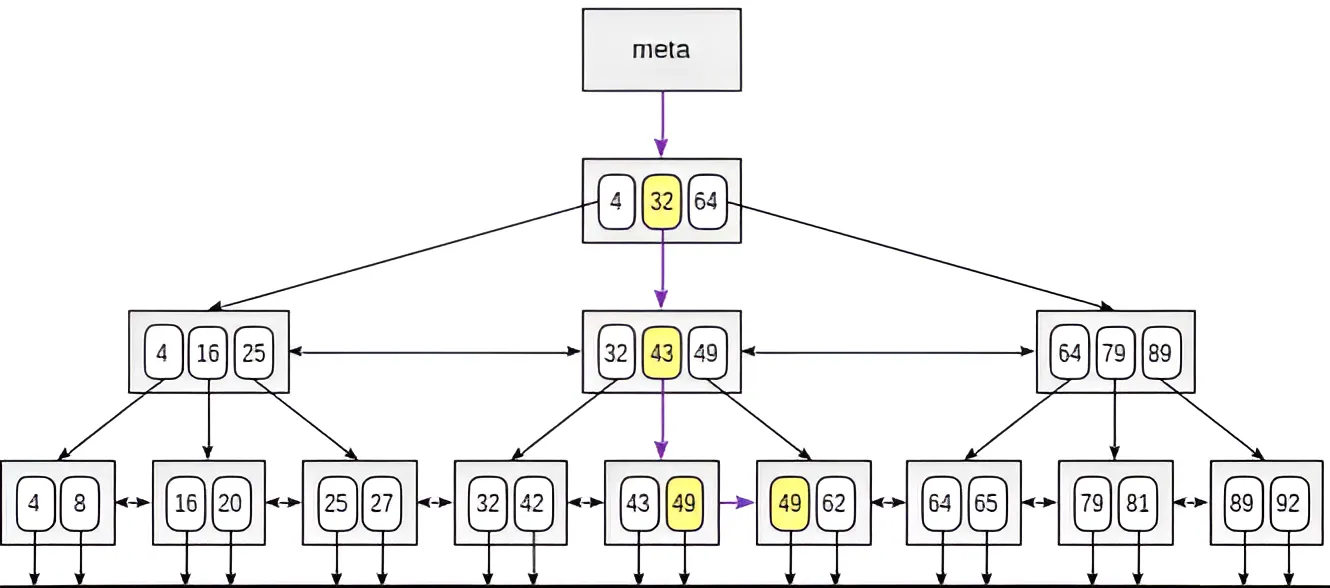
\includegraphics[width=0.9\textwidth]{images/b-tree/equal.png}
\end{frame}

\begin{frame}
  \frametitle{B-Tree индекс: поиск по неравенству}

  \centering
  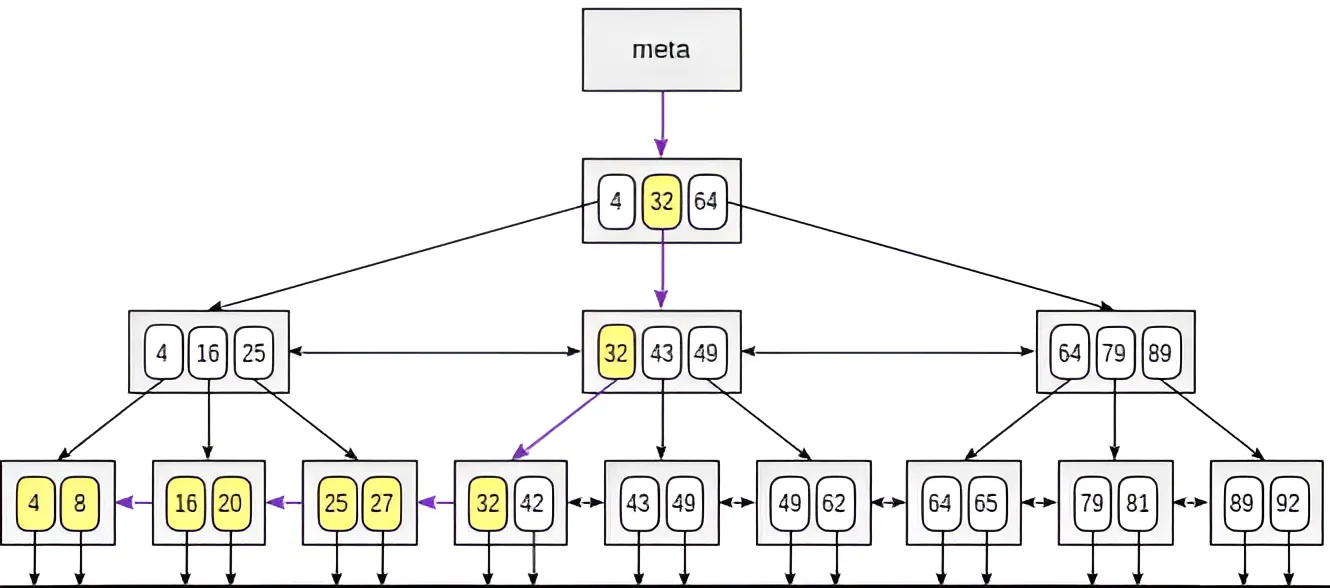
\includegraphics[width=0.9\textwidth]{images/b-tree/less.png}
\end{frame}

\begin{frame}[fragile]
  \begin{center}
    {\Large \textbf{B-Tree индекс: синтаксис}}

    \vspace*{1em}

    \begin{cminted}{sql}
      CREATE INDEX index_name ON table_name USING btree (column_name);
    \end{cminted}

    \vspace*{1em}

    или просто

    \vspace*{1em}

    \begin{cminted}{sql}
      CREATE INDEX index_name ON table_name (column_name);
    \end{cminted}
  \end{center}
\end{frame}

\begin{frame}
  \frametitle{B-Tree индекс: свойства}

  Поддерживает:
  \begin{itemize}
    \item упорядоченные данные;
    \item уникальные индексы;
    \item создание индекса по нескольким столбцам;
    \item частичные индексы;
    \item индексное сканирование, сканирование битовой карты и исключительно
    индексное сканирование;
    \item работу с NULL.
  \end{itemize}
\end{frame}


\begin{frame}
  \vspace*{1em}
  \begin{center}
    {\LARGE \textbf{B-Tree индекс: когда использовать?}}

    \vspace*{1em}

    В большинстве случаев, если данные не являются специфичными.
  \end{center}
\end{frame}

\begin{frame}
  \vspace*{1em}
  \begin{center}
    {\huge \textbf{Hash индекс}}
  \end{center}
\end{frame}

\begin{frame}
  \frametitle{Hash индекс: устройство}

  \centering
  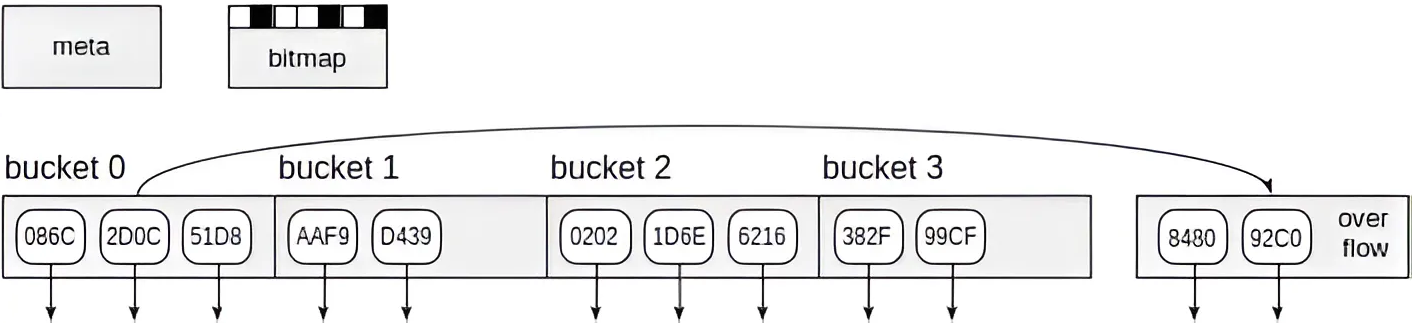
\includegraphics[width=0.9\textwidth]{images/hash/buckets.png}
\end{frame}

\begin{frame}[fragile]
  \begin{center}
    {\Large \textbf{Hash индекс: синтаксис}}

    \vspace*{1em}

    \begin{cminted}{sql}
      CREATE INDEX index_name ON table_name USING hash (column_name);
    \end{cminted}
  \end{center}
\end{frame}

\begin{frame}
  \frametitle{Hash индекс: свойства}

  Поддерживает:
  \begin{itemize}
    \item частичные индексы;
    \item индексное сканирование и сканирование битовой карты.
  \end{itemize}

  Не поддерживает:
  \begin{itemize}
    \item упорядоченные данные;
    \item уникальные индексы;
    \item исключительно индексное сканирование;
    \item создание индексов по нескольким столбцам;
    \item работу с NULL.
  \end{itemize}
\end{frame}

\begin{frame}
  \vspace*{1em}
  \begin{center}
    {\LARGE \textbf{Hash индекс: когда использовать?}}

    \vspace*{1em}

    Hash индекс стоит использовать, если необходимо иметь достаточно быстрый
    поиск и при этом использовать как можно меньше памяти на сам индекс.
  \end{center}
\end{frame}

\begin{frame}
  \vspace*{1em}
  \begin{center}
    {\huge \textbf{GiST индекс}}

    \vspace*{1em}

    Generalized Search Tree
  \end{center}
\end{frame}

\begin{frame}[fragile]
  \begin{center}
    {\Large \textbf{GiST индекс: синтаксис}}

    \vspace*{1em}

    \begin{cminted}{sql}
      CREATE INDEX index_name ON table_name USING gist (column_name);
    \end{cminted}
  \end{center}
\end{frame}

\begin{frame}
  \frametitle{GiST индекс: свойства}

  Поддерживает:
  \begin{itemize}
    \item создание индекса по нескольким столбцам;
    \item частичные индексы;
    \item индексное сканирование, сканирование битовой карты и исключительно
    индексное сканирование;
    \item полнотекстовый поиск.
    \item работу с NULL.
  \end{itemize}

  Не поддерживает:
  \begin{itemize}
    \item упорядоченные данные;
    \item уникальные индексы.
  \end{itemize}
\end{frame}


\begin{frame}
  \vspace*{1em}
  \begin{center}
    {\LARGE \textbf{GiST индекс: когда использовать?}}

    \vspace*{1em}
  \end{center}

  GiST индекс стоит использовать, если необходимо работать с:
  \begin{itemize}
    \item пространственными данными: географические местоположения,
    геометрические фигуры и т. п;
    \item с запросами по диапазонам, например для дат или числовых значений;
    \item полнотекстовым поиском.
  \end{itemize}
\end{frame}

\begin{frame}
  \vspace*{1em}
  \begin{center}
    {\huge \textbf{SP-GiST индекс}}

    \vspace*{1em}

    Space Partitioning Generalized Search Tree
  \end{center}
\end{frame}

\begin{frame}[fragile]
  \begin{center}
    {\Large \textbf{SP-GiST индекс: синтаксис}}

    \vspace*{1em}

    \begin{cminted}{sql}
      CREATE INDEX index_name ON table_name USING spgist (column_name);
    \end{cminted}
  \end{center}
\end{frame}

\begin{frame}
  \frametitle{SP-GiST индекс: свойства}

  Поддерживает:
  \begin{itemize}
    \item частичные индексы;
    \item индексное сканирование, сканирование битовой карты и исключительно
    индексное сканирование;
    \item работу с NULL.
  \end{itemize}

  Не поддерживает:
  \begin{itemize}
    \item упорядоченные данные;
    \item создание индекса по нескольким столбцам;
    \item уникальные индексы.
  \end{itemize}
\end{frame}

\begin{frame}
  \vspace*{1em}
  \begin{center}
    {\LARGE \textbf{SP-GiST индекс: когда использовать?}}

    \vspace*{1em}

    SP-GiST индекс стоит использовать для данных, которые имеют естественную
    группировку элементов и несбалансированную древовидную структуру.
  \end{center}
\end{frame}

\begin{frame}
  \vspace*{1em}
  \begin{center}
    {\huge \textbf{GIN индекс}}

    \vspace*{1em}

    Generalized Inverted Index
  \end{center}
\end{frame}

\begin{frame}[fragile]
  \begin{center}
    {\Large \textbf{GIN индекс: синтаксис}}

    \vspace*{1em}

    \begin{cminted}{sql}
      CREATE INDEX index_name ON table_name USING gin (column_name);
    \end{cminted}
  \end{center}
\end{frame}

\begin{frame}
  \frametitle{GIN индекс: свойства}

  Поддерживает:
  \begin{itemize}
    \item создание индекса по нескольким столбцам;
    \item сканирование битовой карты;
    \item полнотекстовый поиск.
    \item работу с массивами и JSONB.
  \end{itemize}

  Не поддерживает:
  \begin{itemize}
    \item упорядоченные данные;
    \item частичные индексы;
    \item уникальные индексы;
    \item индексное и исключительно индексное сканирование;
    \item работу с NULL.
  \end{itemize}
\end{frame}

\begin{frame}
  \vspace*{1em}
  \begin{center}
    {\LARGE \textbf{GIN индекс: когда использовать?}}

    \vspace*{1em}

    GIN индекс стоит использовать для данных, к которым применяется
    полнотекстовый поиск.
  \end{center}
\end{frame}

\begin{frame}
  \vspace*{1em}
  \begin{center}
    {\huge \textbf{GIN или GiST?}}

    \vspace*{1em}

    Для полнотекстового поиска
  \end{center}
\end{frame}

\begin{frame}
  \vspace*{1em}
  \begin{center}
    {\huge \textbf{BRIN индекс}}

    \vspace*{1em}

    Block Range Index
  \end{center}
\end{frame}

\begin{frame}
  \frametitle{BRIN индекс: устройство}

  \centering
  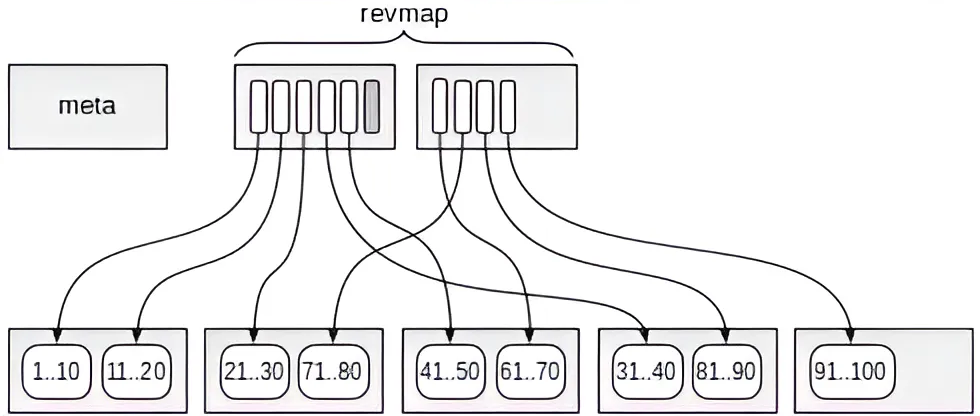
\includegraphics[width=0.8\textwidth]{images/brin/blocks.png}
\end{frame}

\begin{frame}[fragile]
  \begin{center}
    {\Large \textbf{BRIN индекс: синтаксис}}

    \vspace*{1em}

    \begin{cminted}{sql}
      CREATE INDEX index_name ON table_name USING brin (column_name);
    \end{cminted}
  \end{center}
\end{frame}

\begin{frame}
  \frametitle{BRIN индекс: свойства}

  Поддерживает:
  \begin{itemize}
    \item создание индекса по нескольким столбцам;
    \item сканирование битовой карты;
    \item работу с NULL.
  \end{itemize}

  Не поддерживает:
  \begin{itemize}
    \item упорядоченные данные;
    \item частичные индексы;
    \item уникальные индексы;
    \item индексное и исключительно индексное сканирование.
  \end{itemize}
\end{frame}

\begin{frame}
  \vspace*{1em}
  \begin{center}
    {\LARGE \textbf{BRIN индекс: когда использовать?}}

    \vspace*{1em}

    BRIN индекс следует использовать для очень больших упорядоченных наборов
    данных, таких как почтовые индексы или даты.
  \end{center}
\end{frame}

\begin{frame}
  \frametitle{Резюмируя}

  Индекс --- это некоторая структура данных, которая повышает скорость операций
  поиска данных в таблице БД. При этом взамен требует определенных затрат на
  свое поддержание. Поэтому индексы нужно использовать с умом.

  \vspace*{1em}

  В PostgreSQL существует большое количество различных индексов. Чтобы индексы
  работали хорошо на вашем типе данных, нужно понимать, для каких целей
  используется тот или иной индекс.

  \vspace*{1em}

  Проверить, работает ли индекс для определенного запроса, всегда можно с
  помощью оператора EXPLAIN.
\end{frame}

\begin{frame}
  \vspace*{1em}
  \begin{center}
    {\huge \textbf{Приятного использования индексов \\ в PostgreSQL}}
  \end{center}
\end{frame}

\end{document}
